\documentclass[11pt]{article}
\usepackage{mathptmx}
\usepackage[margin=0.85in]{geometry}
\usepackage{setspace}
\usepackage{amsmath}
\usepackage{booktabs}
\usepackage{parskip}
\usepackage{enumitem}
\usepackage{tabularx}
\usepackage{pgfplots}
\pgfplotsset{compat=1.18}
\usepackage{hyperref}
\hypersetup{colorlinks=true, linkcolor=black, urlcolor=blue}

\setlength{\parskip}{4pt}
\singlespacing

\begin{document}

\section*{IEEE 14-Bus Battery Siting --- Model Reference}
\addcontentsline{toc}{section}{IEEE 14-Bus Battery Siting --- Model Reference}

\tableofcontents
\newpage

% ============================================================
\section{Use Case Overview}

\begin{itemize}[noitemsep]
  \item \textbf{Network:} IEEE 14-bus, 20 branches, 5 generators (MATPOWER case14)
  \item \textbf{New load:} 200 MW flat AI datacenter added at Bus 4
  \item \textbf{Batteries:} 4 units (50 MW / 200 MWh each), placement to be optimised
  \item \textbf{Search space:} C(14,4) = 1,001 candidate placements
  \item \textbf{Objective:} minimise total 24-hour system dispatch cost
  \item \textbf{Horizon:} single 24-hour day, hourly resolution
  \item \textbf{Power flow:} DC approximation (PTDF-based, lossless, no reactive power)
  \item \textbf{Source:} \url{https://github.com/Square-Peg-Technologies/square-peg-quantum-challenge}
\end{itemize}

\subsection*{Key Files and Variables}

\noindent\resizebox{\linewidth}{!}{%
\begin{tabular}{lll}
\toprule
File & Variable / Function & Description \\
\midrule
\texttt{ieee14.py}        & \texttt{Case}                & Grid object: PTDF, fbar, power\_demand \\
                           & \texttt{Case.factors}        & 24-hour demand multipliers (list of 24) \\
                           & \texttt{CaseDescription.fbar}& Branch flow limits (MW), 20 elements \\
                           & \texttt{CaseDescription.branch} & Branch r, x, b, ratio data \\
                           & \texttt{CaseDescription.bus} & Bus Pd, Qd base values \\
\midrule
\texttt{assets.py}        & \texttt{GENERATORS}          & List of 5 generator dicts (bus, Pmin, Pmax, cost) \\
                           & \texttt{BATTERIES}           & List of 4 battery dicts (power\_mw, capacity\_mwh, efficiency, init\_soc) \\
                           & \texttt{DATACENTER\_BUS}     & None (base case, no datacenter) \\
                           & \texttt{DATACENTER\_MW}      & 0.0 (base case) \\
\midrule
\texttt{assets\_dc\_bus4.py} & \texttt{DATACENTER\_BUS}  & 4 (active scenario) \\
                           & \texttt{DATACENTER\_MW}      & 200.0 \\
\midrule
\texttt{locations.py}     & \texttt{GENERATOR\_LOCATIONS}& Dict \{gen\_index: bus\} \\
                           & \texttt{BATTERY\_LOCATIONS}  & Placeholder; overridden by solver \\
\midrule
\texttt{site\_datacenter.py} & ---                       & Sweeps all 14 buses as datacenter locations, writes assets\_dc files \\
\midrule
\texttt{solvers/uc.py}    & \texttt{run\_uc()}           & UC + ED (CVXPY/SCIP); fixed placement in, cost out \\
\texttt{solvers/ed.py}    & \texttt{run\_ed()}           & ED only (CVXPY/HiGHS), continuous, no binary \\
\texttt{solvers/siting\_benders.py} & \texttt{run\_siting\_benders()} & Benders decomposition siting (classical) \\
\texttt{solvers/siting\_mip.py} & \texttt{run\_siting\_mip()} & Joint siting + UC MILP, single SCIP solve \\
\midrule
\texttt{solvers/quantum\_siting.py} & \texttt{run\_quantum\_siting()} & Full hybrid pipeline: quantum sieve + classical refinement \\
                           & \texttt{build\_proxy\_cost\_fn()} & Builds $Q(u,s)$ proxy for COBYLA/VQA loop \\
                           & \texttt{build\_butterfly\_ansatz()} & VQA circuit (butterfly ansatz, $L$ layers) \\
                           & \texttt{run\_vqa\_qiskit()}  & Qiskit Aer VQA: COBYLA + final sample \\
                           & \texttt{run\_dwave\_sa()}    & D-Wave simulated annealing (BQM-based) \\
                           & \texttt{compute\_congestion\_signal()} & Per-bus relief signal: PTDF $\times$ shadow prices \\
                           & \texttt{evaluate\_candidates()} & Parallel classical UC/ED eval of quantum candidates \\
\bottomrule
\end{tabular}%
}

% ============================================================
\section{Network: IEEE 14-Bus}

\subsection{Bus Data}

\begin{center}
\begin{tabular}{rlrrl}
\toprule
Bus & Type & Base Pd (MW) & Base Qd (MVAr) & Notes \\
\midrule
1  & Slack (3) & 0.0  & 0.0  & Generator only \\
2  & PV (2)    & 21.7 & 12.7 & Generator + load \\
3  & PV (2)    & 94.2 & 19.0 & Generator + load \\
4  & PQ (1)    & 47.8 & -3.9 & Load only; datacenter bus \\
5  & PQ (1)    & 7.6  & 1.6  & \\
6  & PV (2)    & 11.2 & 7.5  & Generator + load \\
7  & PQ (1)    & 0.0  & 0.0  & Transit bus \\
8  & PV (2)    & 0.0  & 0.0  & Generator only \\
9  & PQ (1)    & 29.5 & 16.6 & Shunt cap 19 MVAr \\
10 & PQ (1)    & 9.0  & 5.8  & \\
11 & PQ (1)    & 3.5  & 1.8  & \\
12 & PQ (1)    & 6.1  & 1.6  & \\
13 & PQ (1)    & 13.5 & 5.8  & \\
14 & PQ (1)    & 14.9 & 5.0  & \\
\midrule
   & \textbf{Total base load} & \textbf{259.0} & & \\
\bottomrule
\end{tabular}
\end{center}

\subsection{Branch Data}

\begin{center}
\small
\begin{tabular}{rlrrrrrl}
\toprule
Br\# & From--To & r (pu) & x (pu) & b (pu) & Limit (MW) & Ratio & Note \\
\midrule
0  & 1--2  & 0.01938 & 0.05917 & 0.0528 & 400  & --    & Strong backbone \\
1  & 1--5  & 0.05403 & 0.22304 & 0.0492 & 120  & --    & \\
2  & 2--3  & 0.04699 & 0.19797 & 0.0438 & 120  & --    & \\
3  & 2--4  & 0.05811 & 0.17632 & 0.0340 & 120  & --    & \\
4  & 2--5  & 0.05695 & 0.17388 & 0.0346 & 120  & --    & \\
5  & 3--4  & 0.06701 & 0.17103 & 0.0128 & 120  & --    & \\
6  & 4--5  & 0.01335 & 0.04211 & 0.000  & 9999 & --    & Local tie (unconstrained) \\
7  & 4--7  & 0.00000 & 0.20912 & 0.000  & 80   & 0.978 & Transformer \\
8  & 4--9  & 0.00000 & 0.55618 & 0.000  & 40   & 0.969 & Transformer; hard bottleneck \\
9  & 5--6  & 0.00000 & 0.25202 & 0.000  & 80   & 0.932 & Transformer; sole path to bus-6 cluster \\
10 & 6--11 & 0.09498 & 0.19890 & 0.000  & 80   & --    & \\
11 & 6--12 & 0.12291 & 0.25581 & 0.000  & 60   & --    & \\
12 & 6--13 & 0.06615 & 0.13027 & 0.000  & 120  & --    & \\
13 & 7--8  & 0.00000 & 0.17615 & 0.000  & 80   & --    & \\
14 & 7--9  & 0.00000 & 0.11001 & 0.000  & 100  & --    & \\
15 & 9--10 & 0.03181 & 0.08450 & 0.000  & 200  & --    & \\
16 & 9--14 & 0.12711 & 0.27038 & 0.000  & 80   & --    & \\
17 & 10--11& 0.08205 & 0.19207 & 0.000  & 80   & --    & \\
18 & 12--13& 0.22092 & 0.19988 & 0.000  & 80   & --    & \\
19 & 13--14& 0.17093 & 0.34802 & 0.000  & 60   & --    & \\
\bottomrule
\end{tabular}
\end{center}

\noindent Key bottlenecks: Branch 8 (4--9, 40 MW) and Branch 9 (5--6, 80 MW) bind at peak and produce non-zero shadow prices with the datacenter at Bus 4.

% ============================================================
\section{Generators}

Five generators. Two cheap units (buses 1, 2 at \$20/MWh), three expensive units (buses 3, 6, 8 at \$40/MWh).

\begin{center}
\begin{tabular}{llrrrr}
\toprule
Name & Bus & Pmin (MW) & Pmax (MW) & cost\_b (\$/MWh) & Startup (\$) \\
\midrule
Gen 1 & 1 & 50  & 332 & 20 & 0 \\
Gen 2 & 2 & 20  & 140 & 20 & 0 \\
Gen 3 & 3 & 20  & 100 & 40 & 0 \\
Gen 4 & 6 & 20  & 100 & 40 & 0 \\
Gen 5 & 8 & 20  & 100 & 40 & 0 \\
\midrule
      &   & \multicolumn{2}{l}{Total installed: 772 MW} & & \\
\bottomrule
\end{tabular}
\end{center}

% ============================================================
\section{Load Profile}

The 24-hour demand shape is defined in \texttt{ieee14.py} (\texttt{Case.factors}), a list of 24 hourly multipliers applied uniformly to all base bus loads. Source: synthetic daily shape scaled to the MATPOWER case14 base load of 259 MW. The 200 MW datacenter load at Bus 4 is added as a flat constant and is not multiplied by these factors. Peak system demand: 363 MW (base) + 200 MW (datacenter) = 563 MW at Hour 13.

\begin{center}
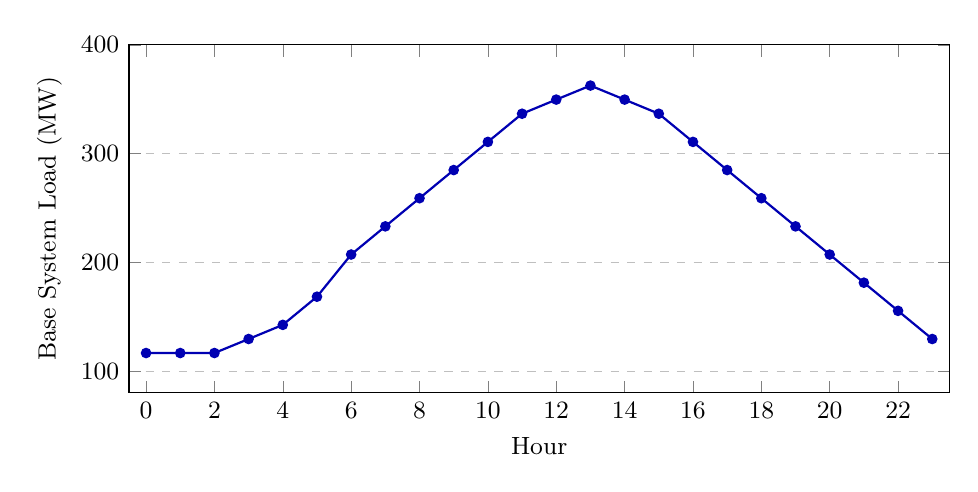
\begin{tikzpicture}
\begin{axis}[
    width=12cm, height=6cm,
    xlabel={Hour},
    ylabel={Base System Load (MW)},
    xmin=-0.5, xmax=23.5,
    ymin=80, ymax=400,
    xtick={0,2,4,6,8,10,12,14,16,18,20,22},
    ymajorgrids=true,
    grid style=dashed,
    tick label style={font=\small},
    label style={font=\small},
]
\addplot[thick, mark=*, mark size=1.5pt, color=blue!70!black] coordinates {
    (0,116.6) (1,116.6) (2,116.6) (3,129.5) (4,142.5) (5,168.4)
    (6,207.2) (7,233.1) (8,259.0) (9,284.9) (10,310.8) (11,336.7)
    (12,349.7) (13,362.6) (14,349.7) (15,336.7) (16,310.8) (17,284.9)
    (18,259.0) (19,233.1) (20,207.2) (21,181.3) (22,155.4) (23,129.5)
};
\end{axis}
\end{tikzpicture}
\end{center}

% ============================================================
\section{Battery Specifications}

Four identical batteries: \textbf{50 MW / 200 MWh, charge efficiency 90\% (discharge lossless), initial SoC 200 MWh (fully charged).} Defined in \texttt{assets.py} as \texttt{BATTERIES}.

% ============================================================
\section{Problem Formulation}
\label{sec:formulation}

\subsection{Objective}

The cost function in \texttt{solvers/uc.py} supports a quadratic-plus-linear form:

\[
\min \sum_{g} \sum_{t=1}^{24} \bigl[ a_g \cdot p_{g,t}^2 + b_g \cdot p_{g,t} + c_g \cdot u_{g,t} + \text{sc}_g \cdot v_{g,t} \bigr]
\]

In this use case, $a_g = 0$ for all generators. The original MATPOWER case14 polynomial gencost data does include small quadratic terms, but this model simplifies to linear-only dispatch costs, consistent with the approach in Aboumrad et al.\ and necessary for keeping the QUBO proxy tractable on near-term hardware. No-load costs $c_g$ and startup costs $\text{sc}_g$ are also zero: startup events are tracked by $v_{g,t}$ (see below) but carry no cost in this formulation.

\subsection{Decision Variables}

\begin{itemize}[noitemsep]
  \item $p_{g,t} \geq 0$: generator output (MW)
  \item $u_{g,t} \in \{0,1\}$: generator commitment (1 = online)
  \item $v_{g,t} \in \{0,1\}$: startup indicator --- equals 1 when generator $g$ transitions from off ($u=0$) at $t-1$ to on ($u=1$) at $t$, enforced by $v_{g,t} \geq u_{g,t} - u_{g,t-1}$. With $\text{sc}_g = 0$ it does not affect the objective but is retained for generality.
  \item $r^+_{b,t} \geq 0$: battery charge (MW)
  \item $r^-_{b,t} \geq 0$: battery discharge (MW)
  \item $\text{SoC}_{b,t} \geq 0$: state of charge (MWh)
  \item $z_{b,t} \in \{0,1\}$: direction flag (1 = charging) --- prevents simultaneous charge and discharge
\end{itemize}

\subsection{Constraints}

\textbf{Generator bounds:}
\[
P^{\min}_g \cdot u_{g,t} \leq p_{g,t} \leq P^{\max}_g \cdot u_{g,t}
\]

\textbf{Power balance} (per hour):
\[
\sum_g p_{g,t} + \sum_b (r^-_{b,t} - r^+_{b,t}) = \sum_i D_{i,t}
\]

where $D_{i,t}$ is bus load at hour $t$ (base load $\times$ factor, plus 200 MW flat at Bus 4).

\textbf{DC line flow limits} (per branch $\ell$, per hour):
\[
-\bar{f}_\ell \leq \sum_i \mathrm{PTDF}_{\ell,i} \cdot \mathrm{net}_{i,t} \leq \bar{f}_\ell
\]

where $\mathrm{net}_{i,t} = \mathrm{injection}_{i,t} - D_{i,t}$.

\textbf{Battery charge/discharge exclusion:}
\[
r^+_{b,t} \leq P^{\mathrm{bat}} \cdot z_{b,t}, \qquad r^-_{b,t} \leq P^{\mathrm{bat}} \cdot (1 - z_{b,t})
\]

\textbf{SoC bounds:} $0 \leq \mathrm{SoC}_{b,t} \leq 200~\mathrm{MWh}$, with $\mathrm{SoC}_{b,0} = 200~\mathrm{MWh}$.

\subsection{Siting Algorithm}

The Benders decomposition (\texttt{siting\_benders.py}) works as follows:

\begin{enumerate}[noitemsep]
  \item \textbf{Master problem} (SCIP MIP): selects which buses to place the 4 batteries on. Binary variables $x_{b,n}$; exactly one bus per battery; symmetry-breaking enforces ascending bus index for identical batteries.
  \item \textbf{Subproblem} (\texttt{run\_uc()}): given a fixed placement, solves the 24-hour UC/ED. Returns total cost $Z$.
  \item \textbf{Cuts:} no-good cuts prevent re-visiting placements. L-shaped optimality cuts $\eta \geq Z \cdot (\sum_{(b,n)\in S^+} x_{b,n} - (M-1))$ bound the master from below.
  \item \textbf{Convergence:} master lower bound $\geq$ best known cost, or time limit.
\end{enumerate}

An alternative joint MILP is in \texttt{siting\_mip.py} (single SCIP solve, big-M linearisation of placement $\times$ dispatch).

% ============================================================
\section{Comparison}

\begin{center}
\begin{tabular}{lrr}
\toprule
Run & Bus placement & 24h cost \\
\midrule
No batteries, no datacenter & --- & \$209,229 \\
No batteries, datacenter at Bus 4 & --- & \$228,429 \\
Quantum (Qiskit Aer) & (2, 4, 6, 7) & \$199,804 \\
Classical (SCIP) & (2, 4, 6, 7) & \$199,804 \\
\bottomrule
\end{tabular}
\end{center}

\noindent Quantum and classical solvers agree on both the optimal placement and cost. Quantum runtime: approximately 2.5 minutes on GPU. Classical solver: \texttt{run\_siting\_benders()} or \texttt{run\_siting\_mip()}.

\end{document}
